\documentclass{article}
\usepackage{amsmath}
\usepackage{url}
\usepackage{graphicx}
\title{Fitting ODE solutions to noisy data by collapsing towards to manifold of solutions}
\author{Harry Braviner}

\date{\today}

\begin{document}
\maketitle

\section{Statement of the problem}

We have a collection of datapoints, $\left\{ \tilde{x}(t_i) \right\}$, and an ODE, $\mathcal{D}\left[ x; t \right] = 0$. We believe that the datapoints \emph{may be} noisy samples from \emph{some} solution to this ODE, but we do \emph{not} have a guess for the intial or bounday conditions. How can we evaluate the goodness-of-fit of this ODE (which we probably cannot solve analytically, and which we do not have initial conditions for) to these datapoints?

Let's simplify the problem space by making two big restrictions:
\begin{enumerate}
\item We only consider second-order ODEs. i.e. the differential operator $\mathcal{D}\left[x ; t \right]$ has the form $\ddot{x}(t) - f\left(x(t), \dot{x}(t), t\right)$.
\item The datapoints are samples from an evenly-spaced discrete grid of times, $t_0, t_1, \dots, t_{N-1}$, where $t_i - t_{i-1} = h$. The samples themselves need not be evenly spaced: e.g. out dataset could consist of $\left\{\tilde{x}(t_0), \tilde{x}(t_1), \tilde{x}(t_2), \tilde{x}(t_50)\right\}$. We also assume that we have at most one samples from any $t_i$. i.e. we never have multiple samples from the same time with different noise components.
\end{enumerate}

I am not concerned at this point about where $f$ comes from.
The motivation for everything in this document is that I would like to be able to modify PySR to search for such an $f$.
Doing so requires%
\footnote{It also requires modifying PySR to output functions of $t$, $x(t)$, and $\dot{x}(t)$, but I believe that is comparatively straightforward: have PySR treat $t$, $x(t)$ and $\dot{x}(t)$ as three dependent variables.}
evaluating the goodness-of-fit of each $f$ to the data, and this work is intended to provide a method of doing so.

The essential idea I shall outline is this: We will approximate the (infinite dimensional) space of function on $\left[t_{\mathrm{start}}, t_{\mathrm{end}} \right]$ by an $N$-dimensional discretization
$$
\left( \hat{x}(t_0), \hat{x}(t_1), \dots, \hat{x}(t_{N-1} \right)
$$
Within this $N$-dimensional space there is some subspace (the \emph{solution space}) that satisfies the ODE.%
\footnote{
And for a one-dimensional second-order ODE this subspace should generally by 2-dimensional.
}
\textbf{We shall collapse the $N$-dimensional discretization onto the solution space \emph{along the path minimizing the MSE of the data}.}
I shall be more precise about what this means in section \ref{sec:method}, after briefly reviewing other work and ideas.

\subsection{Previous work}

I haven't done a very comprehensive literature review, so I can't rule out that someone has done something similar to myself.
However, a little googling hasn't turned up anything identical.
I'll review here what I \emph{did} find, since a lot of this is quite interesting, might provide inspiration along different directions, and I want to at least have it written down for my own purposes.

In \cite{kronberger2019identification} the authors consider symbolic regression of first-order autonomous dynamical systems:
\begin{align}
\dot{x}_1(t) &= f_1\left(x_1, \dots, x_n\right) \nonumber \\
\dot{x}_2(t) &= f_2\left(x_1, \dots, x_n\right) \nonumber \\
 & \vdots \nonumber \\
\dot{x}_n(t) &= f_n\left(x_1, \dots, x_n\right) \nonumber \\
\end{align}
The candidate system, $\left( f_1, f_2, \dots, f_n\right)$, is the output of a genetic algorithm, although it does not appear to be PySR.
The authors use two methods of evaluating the goodness-of-fit of the ODE to the datapoints:
\begin{enumerate}
\item Using the approximate derivative values as a target, i.e.
$$
\mathrm{Loss}(f) = \sum_{i, j} \bigg(f_i\left( x_1(t_j), \dots, x_n(t_j) \right) - \big(x_i(t_{j+1}) - x_i(t_j)\big) \bigg)^2
$$
\item Integrating from the initial values $(x_1(t_0), ..., x_n(t_0))$ using a numerical ODE solver.
\end{enumerate}
The method of \cite{kronberger2019identification} does not appear to allow for noise in the measurements.
The results section shows the method being less successful on motion-captured data vs simulated data, and this supports my belief that this method does not tolerate measurement noise well.
They also assume that their datapoints are evenly spaced in time, although I'm not sure this is necessary. However, for method (1) to work, it is necessary for the spacing between the datapoints to be such that the numerical gradient is a good approximation to the true gradient.

\cite{bongard2007automated} also appears to integrate the candidate ODE from initial conditions that are assumed to be know.
The authors describe a system which not only evaluates candidate dynamical systems, but also suggests new experiments (i.e. initial conditions) that should best disambiguate between currently-strong candidates.
While this is a useful capability, and possibly the reason that the authors assume the initial conditions are known (because you set up the exeriment), it neglects the fact that in reality we never quite set up the system as we intend to.
The paper also assumes that the system is first order.

In \cite{iba2008inference} it is not clear how the authors obtain initial conditions, but I think that they simply take the same initial conditions used to generate the data and pass these, along with the candidate system, to the ODE integrator. Again, this paper condiders first order dynamical systems.

In \cite{d2023odeformer} the authors implement an end-to-end deep learning approach.
Input observations (i.e. $(x_1(t_i), \dots x_n(t_i), t_i)$) are embedded and then passed to a transformer, which outputs $(f_1, \dots, f_n)$ in the form of a string of symbols representing the tree form of the $f$s in prefix notation.
The model is trained on a randomly generated synthetic dataset.
This has the advantage that the target string is known (because it was generated at random), and the input data (the samples) are generated by numerical integration of the $f$.
The authors do consider noisy data and non-uniform spacing ('subsampling').
This paper completely sidesteps the issue of how to evaluate the goodness-of-fit without the underlying initial conditions: we do not have to repeatedly evaluate the goodness-of-fit of $f$s, because we only have a single candidate, the output of the transformer.
Unlike PySR, this method does not produce a Pareto front.

The issue \cite{pysrissue568} on the PySR github repo suggests that, at least as of March 2024, the accepted method for performing SR for an ODE was haveing PySR generate both the ODE and the initial conditions.
This has two issues.
First, the additional time taken to search for initial conditions (and all of the problems I will discuss in the next section regarding sweep-and-shoot approaches).
Secondly, outputting an ODE and an intial condition allows us to test only a single dataset.
We might have multiple timeseries that we believe obey the same ODE with different initial conditions.

In issue \cite{pysrissue732} Miles refers someone looking to so SR on ODEs to \cite{pysrchangenotev1.3.0}, which suggests performing integration of a function by generating data points for the integrand, and then performing SR on candidate expressions for the integral.
Could this method be applied to an ODE (by replacing the dataset generated from the integrand in \cite{pysrchangenotev1.3.0} by the timeseries)?
One limitation of doing so is that we are now searching over the expression for the \emph{solution to} the ODE.
Many physical systems have a simple expression in terms of ODEs, but no closed form solution to that ODE.

\subsection{Alternative methods}

In this section I'm going to outline some alternative methods that seem attractive.

\subsubsection{Extracting $\dot{x}(t)$ from the data}

Several of the papers described above evaluate $f$ directly as the degree of disagreement between $f(x(t))$ and $\dot{x}(t)$ as measured from the data.
Even if the data has zero noise, the descretization of the time-sampling can cause considerable error in the approximation (see figure \ref{fig:deriv_from_samples}), and the addition of noise makes the error much worse (see figure \ref{fig:deriv_from_noisy_samples}).
The method I outline in the note should be able to handle much sparser and noisier data.

\begin{figure}
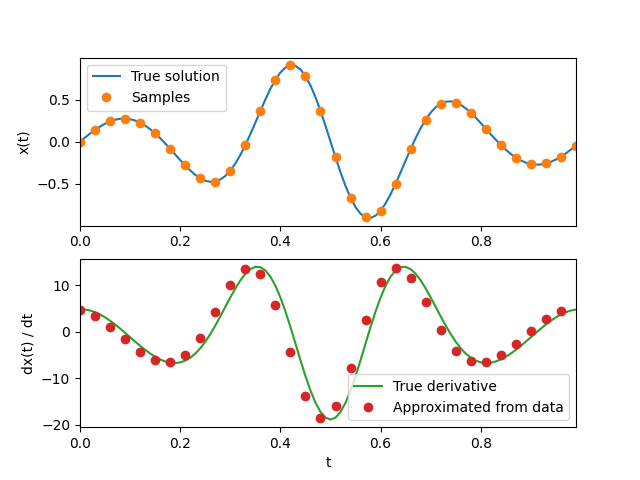
\includegraphics{images/alternative_methods/deriv_from_samples.png}
\centering
\caption{Forward numerical derivative, $\left(x(t_{i+1}) - x(t_i)\right)/\left(t_{i+1} - t_i\right)$} from sampled data. There is an error, with the derivative being shifted left, even though the points are densely spaced.
\label{fig:deriv_from_samples}
\end{figure}

\begin{figure}
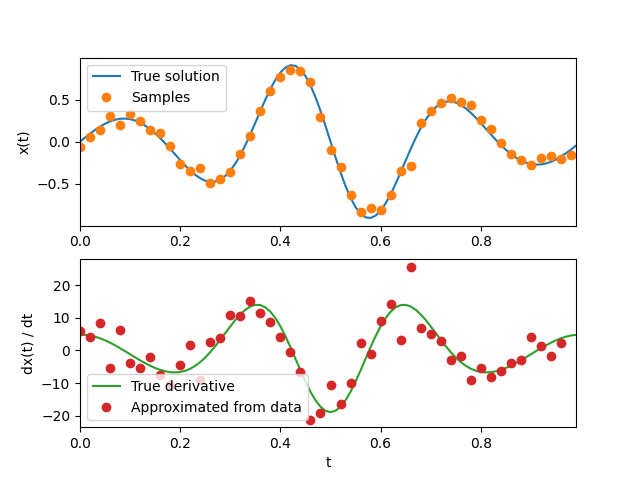
\includegraphics{images/alternative_methods/deriv_from_noisy_samples.png}
\centering
\caption{Forward numerical derivative, $\left(x(t_{i+1}) - x(t_i)\right)/\left(t_{i+1} - t_i\right)$} from sampled data with Gaussian noise with $\sigma = 0.05$. The error is considerably worse than in figure \ref{fig:deriv_from_samples}.
\label{fig:deriv_from_noisy_samples}
\end{figure}

%% FIXME - shooting and sweeping method. Downsides: double well example. High-dimensional search space.
%% FIXME - treating the first and last points as 'correct' and performing relaxation. Noise is an issue. double-well example also provides a case where it works poorly.
%% FIXME - smoothing over the points with some kind of kernel. Necessitates a choice of smoothing length-scale.


\section{Collapse method in detail}
\label{sec:method}

%%FIXME
%and the derivatives by
%$$
%\hat{\ddot{x}}(t_i) = h^{-2} \left( \hat{x}(t_{i-1}) - 2 \hat{x}(t_i) + \hat{x}(t_{i+1}) \right)
%$$
%and%
%\footnote{
%We could instead use the backward derivative, $\hat{\dot{x}}(t_i) = h^{-1} \left( \hat{x}(t_{i}) -  \hat{x}(t_{i-1})\right)$. I do not think this should make a difference, but I have added an option to do so in my code.
%}
%$$
%\hat{\dot{x}}(t_i) = h^{-1} \left( \hat{x}(t_{i+1}) -  \hat{x}(t_i)\right)
%$$

\bibliographystyle{plain}
\bibliography{ode_collapser}

\end{document}


